\chapter{Implementierung}

\section{Laden und Aufbereitung der MNIST Daten}
Für das neuronale Netzwerk zur Erkennung von hangeschriebenen Zeichen werden Test- und Trainingsdaten der MNIST Datenbank genutzt. Die Datensätze können unter folgender Adresse gefunden werden: 
\\[0.2cm]
\hspace*{1.3cm}
\href{http://yann.lecun.com/exdb/mnist/}{http://yann.lecun.com/exdb/mnist/}.
\\[0.2cm]
Da der MNIST Datensatz lediglich in Form von Binärdateien vorliegt und es in der aktuellen Version von SetlX nicht möglich ist Binärdateien zu lesen, wurde statt dem original Datensatz der umgewandelte Datensatz in Form einer CSV-Datei verwendet. Die Dateien können hier heruntergeladen werden:
\\[0.2cm]
\hspace*{1.3cm}
\href{https://pjreddie.com/projects/mnist-in-csv/}{https://pjreddie.com/projects/mnist-in-csv/}.
\\[0.2cm]
Die Verwendung des CSV-Formats führt dazu, dass die Größe der Datensätze auf Grund fehlender Komprimierungen ansteigt. Ebenso wird das Einlesen der Datensätze langsamer, was an der eigentlichen Funktion des neuronalen Netzes allerdings nichts ändert und somit für dieses Projekt vertretbar ist. Eine Option das erste Problem zu umgehen wäre die Komprimierung in das Zip-Format und die Dekomprimierung zu Beginn des Startens des Programms. Da SetlX keine Unzip-Funktion für Dateien bietet, müsste hierbei allerdings Kenntnis über das jeweils vom Benutzer verwendete Betriebssystem gegeben sein und ebenso ob und wenn ja welches Programm hierfür zur Verfügung steht. Bei der Festlegung auf ein ein Kommandozeilen-Befehl (z.B. "gunzip" oder "unzip" für Linux-basierte PCs) würde somit die Betriebssystemunabhängigkeit verloren gehen.\\
Verwendet werden die CSV-Dateien $\mathtt{mnist\_test.csv}$ und $\mathtt{mnist\_train.csv}$. Die Traingsdaten umfassen insgesamt 60.000 Datensätze und die Testdaten 10.000 Datensätze. 
Die einzelnen Datensätze, also die handgeschriebenen Zeichen, sind in den Dateien in folgendem Format gespeichert:
\begin{center}
	$\mathtt{label, pixel1, pixel2, pixel3, ..., pixel784}$ \\
	$\mathtt{label, pixel1, pixel2, pixel3, ..., pixel784}$ \\
	...
\end{center}
Das heißt, in jeder Zeile befinden sich alle Daten zu einer Ziffer. Der erste Wert gibt den jeweiligen Wert an (z.B. 5) und darauf folgend befinden sich alle Pixel der Ziffer mit deren jeweiligen Graustufenwerten. Die Pixel werden der Reihe nach abgespeichert, wobei die "Leserichtung" einer Ziffer von links nach rechts und dann von oben nach unten ist.\\ \\
Um die Datensätze nun in SetlX importieren zu können, wird die Datei $\mathtt{csv\_loader.stlx}$ verwendet. Wird die Datei im SetlX-Interpreter ausgeführt, so liest sie die CSV-Dateien der Test- und Trainingsdaten (die Dateien müssen im selben Verzeichnis liegen und den oben erwähnten Namen haben) und speichert die Daten in den Variablen $\mathtt{test\_data}$ sowie $\mathtt{training\_data}$. Die Testdaten sind hierbei als Liste von Paaren in folgender Form abgelegt: \\
\hspace*{0.3cm}
$
\begin{array}[t]{lcll}
	[ \\[0.1cm]
	
	\hspace*{0.5cm}
	\begin{array}[t]{lcll}
    	[\mathtt{pixels},\ \mathtt{label}], \\[0.1cm]
    	[\mathtt{pixels},\ \mathtt{label}], \\[0.1cm]
    	... \\[0.1cm]
    \end{array}
    \\[0.1cm]
    
    ] \\[0.1cm]
\end{array}
$
\\[0.0cm]

\noindent
Hierbei ist $\mathtt{pixels}$ eine Liste mit Integer Werten zwischen 0 und 255. Der Wert des Zeichens wird in $\mathtt{label}$ als Integer gespeichert. \\ 
Die Trainingsdaten sind prinzipiell nach dem gleichen Prinzip aufgebaut, allerdings wird hier für spätere Auswertungszwecke der Wert der Ziffer nicht als konkrete Zahl gespeichert, sondern in vektorisierter Form. Der vektorisierte Wert einer Zahl wird hier durch einen Vektor dargestellt, dessen Inhalt immer 0 ist, außer an der $\mathtt{label+1}$-ten Stelle. Dies entspricht dann genau der Form der Ausgabe des Netzwerkes. Beispielhaft würde eine Ziffer mit dem Wert $7$ als folgender Vektor dargestellt werden: \\
$<<0\ 0\ 0\ 0\ 0\ 0\ 0\ 1\ 0\ 0>>$ \\

\noindent
Auf eine genaue Beschreibung der Implementierung des Ladevorgangs wird in dieser Studienarbeit verzichtet, da hierbei keine komplexen Funktionen angewandt wurden und das Verfahren nicht relevant für das Verständnis neuronaler Netze an sich ist.

\section{Implementierung des neuronalen Netzes}
Dieser Abschnitt beschreibt die eigentliche Implementierung des neuronalen Netzwerkes zur Erkennung von handgeschriebenen Ziffern in SetlX. Um den Code möglichst kompakt zu halten, wurden die in den Originaldateien enthaltenen Kommentarzeilen in dieser Seminararbeit zum größten Teil entfernt.
Bei der Umsetzung des Netzwerkes in SetlX wird der Stochastic Gradient Descent (SGD) Algorithmus als Lernmethode des Netzwerkes benutzt. Die im vorherigen Kapitel importierten Daten des MNIST-Datensatzes dienen als Grundlage der Ziffernerkennung. 
Das Netzwerk wird als Klasse in SetlX angelegt und enthält die folgenden Membervariablen:

\begin{enumerate}
\item $\mathtt{mNumLayers}$: Anzahl der Schichten des aufzubauenden Netzwerkes 
\item $\mathtt{mSizes}$: Aufbau des Netzwerkes in Listenform. Bsp.: $[784, 30, 10]$ beschreibt ein Netzwerk mit 784 Eingabefeldern, 30 Neuronen in der zweiten Schicht und 10 Ausgabe-Neuronen
\item $\mathtt{mBiases}$: Alle Vorbelastungen des Netzwerkes (genauer Aufbau wird im Folgenden erläutert)
\item $\mathtt{mWeights}$: Alle Gewichte des Netzwerkes (genauer Aufbau wird im Folgenden erläutert)
\end{enumerate}

\noindent
Die Initialisierung des Netzwerkes zur Ziffernerkennung erfolgt durch folgende Befehle:
\begin{Verbatim}[ frame         = lines, 
                  framesep      = 0.3cm, 
                  firstnumber   = 1,
                  labelposition = bottomline,
                  numbers       = left,
                  numbersep     = -0.2cm,
                  xleftmargin   = 0.8cm,
                  xrightmargin  = 0.8cm,
                ]
    net := network([784, 30, 10]);
    net.init();
\end{Verbatim}
Als Übergabeparameter bei der Erstellung eines Netzwerk-Objektes wird die Struktur des Netzwerkes in Form einer Liste übergeben. Diese wird dann lediglich $\mathtt{mSizes}$ zugeordnet und basierend hierrauf wird $\mathtt{mNumLayers}$ ermittelt.
Die $\mathtt{init()}$-Funktion der $\mathtt{network}$-Klasse wird verwendet um die Gewichte und Vorbelastungen des Netzwerkes initial zufällig zu belegen. Hiermit werden Ausgangswerte gesetzt, welche später durch das Lernen des Netzwerkes angepasst werden.
Im Folgenden sind die verwendeten Funktionen, welche während der Gewichts- und Vorbelastungs-Initialisierung verwendet werden, zu sehen. Nachfolgend werden die Funktionen zur Initialisierung aus Abbildung \ref{fig:init} erläutert.
\begin{figure}
\begin{Verbatim}[ frame         = lines, 
                  framesep      = 0.3cm, 
                  firstnumber   = 1,
                  labelposition = bottomline,
                  numbers       = left,
                  numbersep     = -0.2cm,
                  xleftmargin   = 0.8cm,
                  xrightmargin  = 0.8cm,
                ]
    init := procedure() {
        computeRndBiases();
        computeRndWeights();
    };
    computeRndBiases := procedure() {
        this.mBiases := [0] + [ 
            computeRndMatrix(1, mSizes[i]) : i in [2..mNumLayers] 
        ];
    };
    computeRndWeights := procedure() {
        this.mWeights := [0] + [ 
            computeRndMatrix(mSizes[i], mSizes[i+1]) : i in [1..mNumLayers-1] 
        ];
    };
    computeRndMatrix := procedure(row, col) {
        return la_matrix([
            [ ((random()-0.5)*2)/28 : p in [1..row] ] : q in [1..col]
        ]);
    };
\end{Verbatim}
\vspace*{-0.3cm}
\caption{Initialisierungsfunktionen des Netzwerkes}
\label{fig:init}
\end{figure}

\begin{enumerate}
\item $\mathtt{init()}$: In der Funktion werden die Vorbelastungen und Gewichtungen des Netzwerkes zu Beginn initialisiert
\item $\mathtt{computeRndBiases()}$: Die Funktion befüllt die Variable mBiases mit zufälligen Werten. Der für das Netzwerk benötigte Aufbau der Vorbelastungen entspricht folgender Form: \\
$[\ 0,\\ 
<<\ <<\mathtt{Bias\_Schicht2\_Neuron1}>>\ <<\mathtt{Bias\_Schicht2\_Neuron2}>>\ ...\ >>, \\
<<\ <<\mathtt{Bias\_Schicht3\_Neuron1}>>\ ...\ >>, \\
 ...\ ]$ \\
Das heißt es kann auf die Vorbelastungen mit folgendem Schema in SetlX zugegriffen werden: \\
\begin{center}
	$\mathtt{mBiases[Schicht][Neuron][1]}$
\end{center}
Hierbei ist zu beachten, dass der letzte Index immer 1 ist, da jedes Neuron nur eine einzige Vorbelastung besitzt und die Vorbelastungen als Matrix abgelegt werden. Die Verwendung des Matrix-Datentyps wurde bewusst, auf Grund späterer Berechnungen mit Hilfe der $\mathtt{la\_hadamard()}$-Funktion, gewählt. Da es sich bei der Eingabe-Schicht des Netzwerkes nicht um Sigmoid-Neuronen handelt, sondern lediglich um Eingabewerte, werden hierfür keine Vorbelastungen benötigt. Deshalb wird bei der Erstellung der zufälligen Vorbelastungen nur $[2..\mathtt{mNumLayers}]$ (also alle Schichten außer der Ersten) betrachtet und die erste Schicht wird in Form einer 0 am Anfang der Liste platziert.
\item $\mathtt{computeRndWeights()}$: Diese Funktion ist equivalent zu der Vorbelastungs-Funktion, lediglich wird die Struktur der Gewichte mit folgenden Zugriffmsmöglichkeiten angelegt: \\
\begin{center}
	$\mathtt{mWeights[Schicht][Neuron][Gewicht]}$
\end{center}
\item $\mathtt{computeRndMatrix()}$: Diese Hilfsfunktion dient zur Erstellung der Struktur der Gewichte und Vorbelastungen in den zuvor vorgestellten Funktionen. Die Funktion enthält als Parameter die Anzahl von Reihen und Spalten. Zurückgegeben wird die zugehörige Matrix mit zufälligen Werten zwischen $-1/28$ und $1/28$. Der Wert 28 ergibt sich aus der Größe des Eingabevektors (28x28 Pixel). \\
Bsp.: $s := 1, 2\ \rightarrow\ <<\ <<x>>\ <<y>>\ >>$ und $s := [2,1]\ \rightarrow\ <<\ <<x\ y>>\ >>$
\end{enumerate}

\noindent
Sei nun $W$ die Liste aller Gewichtsmatrizen des Netzwerkes und $B$ die Liste aller Vorbelastungsmatrizen. Die Elemente der Vorbelastungsliste könnten auch als Vektor abgespeichert werden, werden aber wie oben erwähnt auf Grund später benötigter Berechnungen als Matrix abgelegt. $\mathbf{a}$ bezeichnet den Aktivierungsvektor der vorherigen Schicht, also deren Ausgabe (zu Beginn also die Pixel der Eingabe). Nach Gleichung \ref{eq:feedforward2} zur Berechnung einer Sigmoid-Ausgabe lässt sich nun folgende Formel aufstellen: 
\begin{equation}\label{eq:feedforward_impl}
	\mathbf{a}^{(l)} = S(W^{(l)}\cdot \mathbf{a}^{(l-1)} + B^{(l)})
\end{equation}
\noindent
Hierbei bezeichnet $\mathbf{a}^{(l)}$ den Ausgabe-Vektor der aktuellen Schicht, welcher dann der nächsten Schicht weitergeleitet wird (feedforwarding). In Abbildung \ref{fig:feedforward_sigmoid} sind die Implementierungen der Sigmoid-Funktionen sowie dem Feedforwarding zu sehen.
\begin{figure}
\begin{Verbatim}[ frame         = lines, 
                  framesep      = 0.3cm, 
                  firstnumber   = 1,
                  labelposition = bottomline,
                  numbers       = left,
                  numbersep     = -0.2cm,
                  xleftmargin   = 0.8cm,
                  xrightmargin  = 0.8cm,
                ]
    feedforward := procedure(a) {
        for( i in {2..#mBiases} ) { 
            a := sigmoid( mWeights[i]*a + mBiases[i] );
        }
        return a;
    };                            
    sigmoid := procedure(z) {
        return la_vector([ 1.0/(1.0 + exp(- z[i] )) : i in [1..#z] ]);
    };
    sigmoid_prime := procedure(z) {
        s := sigmoid(z); 
        return la_matrix([ [ s[i] * (1 - s[i]) ] : i in [1..#s] ]);
    };
\end{Verbatim}
\vspace*{-0.3cm}
\caption{Feedforward und Sigmoid-Funktionen}
\label{fig:feedforward_sigmoid}
\end{figure}
\begin{enumerate}
\item $\mathtt{feedforward(a)}$: Anwendung der Gleichung \eqref{eq:feedforward_impl} auf alle Schichten des Netzwerkes mit Ausnahme der Eingabeschicht (da hier keine Gewichte und Vorbelastungen vorhanden sind) angewandt. Zurückgegeben wird die resultierende Ausgabe jedes Neurons der letzten Schicht in vektorisierter Form.
\item $\mathtt{sigmoid(z)}$: Diese Funktionen nimmt einen Vektor $\mathtt{z}$ und berechnet mit Hilfe der Sigmoid-Formel (siehe Kapitel \ref{chap:sigmoid}) die Ausgabe der Neuronen in vektorisierter Form.
\item $\mathtt{sigmoid\_prime(z)}$: Für einen gegebenen Vektor $\mathtt{z}$ wird die Ableitung der Sigmoid-Funktion (nach Formel \eqref{eq:sigmoidPrime}) berechnet und in Form einer Matrix (Matrix-Form auf Grund späterer Berechnung mit $\mathtt{la\_hadamard()}$) zurückgegeben.
\end{enumerate}
\noindent
Die Feedforward-Funktion dient also dazu, die Eingabewerte durch das gesamte Netzwerk durchzureichen und die daraus resultierende Ausgabe zu ermitteln. Als nächstes wird der Algorithmus diskutiert, durch welchem es dem Netzwerk ermöglicht wird zu \glqq lernen\grqq. Hierfür wird der SGD-Algorithmus verwendet. Die Implementierung des SGDs in SetlX ist in Abbildung \ref{fig:sgd_func} aufgezeigt und wird nun im Detail erläutert.

\begin{figure}
\begin{Verbatim}[ frame         = lines, 
                  framesep      = 0.3cm, 
                  firstnumber   = 1,
                  labelposition = bottomline,
                  numbers       = left,
                  numbersep     = -0.2cm,
                  xleftmargin   = 0.8cm,
                  xrightmargin  = 0.8cm,
                ]
    sgd := procedure(training_data, epochs, mini_batch_size, eta, test_data) {
        if(test_data != null) {
            n_test := #test_data; 		
        }
        n := #training_data;		
        for(j in {1..epochs}) {
            training_data := shuffle(training_data);
            mini_batches := [ 
                training_data[k..k+mini_batch_size-1] : k in [1,mini_batch_size..n] 
            ];		
            for(mini_batch in mini_batches) {
                update_mini_batch(mini_batch, eta);
            } 		
            if(test_data != null) {
                ev := evaluate(test_data);
                print("Epoch $j$: $ev$ / $n_test$");
            }
            else {
                print("Epoch $j$ complete");
            }
        }
    };
\end{Verbatim}
\vspace*{-0.3cm}
\caption{SGD-Funktion}
\label{fig:sgd_func}
\end{figure}
\begin{enumerate}
\item Zeile 1: Übergabeparameter der Funktion sind die Trainingsdatensätze (Liste von Tupeln $\mathtt{[x,y]}$ mit $\mathtt{x}$ als Eingabewerten und $\mathtt{y}$ als gewünschtem Ergebnis), die Anzahl der Epochen (Integer-Wert), die Größe der Mini-Batches (Integer-Wert), die gewünschte Lernrate (Fließkomma-Wert) und den optionalen Testdatensätzen (äquivalenter Aufbau zu Trainingsdaten).
\item Zeile 6: Der nachfolgende Programmcode wird entsprechend der übergebenen Epochenanzahl mehrfach ausgeführt.
\item Zeile 7-10: Zuerst werden alle Trainingsdaten zufällig vermischt und anschließend Mini-Batches (also Ausschnitte aus dem Gesamtdatensatz) der vorher festgelegten Größe aus den Trainingsdaten extrahiert. Somit wird eine zufällige Belegung von Mini-Batches garantiert. Alle Mini-Batches werden in Listenform in der Variablen $\mathtt{mini\_batches}$ gespeichert.
\item Zeile 11-13: Anschließend wird für jeden Mini-Batch aus $\mathtt{mini\_batches}$ eine Iteration des Gradient Descent Algorithmus angewendet. Dies geschieht mit Hilfe der Funktion $\mathtt{update\_mini\_batches}$, welche im nächsten Schritt ausführlicher erläutert wird. Zweck der Funktion ist es die Gewichte und Vorbelastungen des Netzwerkes mit Hilfe einer Iteration des SGD-Algorithmus anzupassen. Die Basis für diese Anpassung liefert der übergebene Mini-Batch und die Lernrate.
\item Zeile 14-20: Dieser Programmcode dient zur Ausgabe auf der Konsole und teilt dem Benutzer die aktuelle Anzahl an korrekt ermittelten Datensätzen der Trainingsdaten nach jeder Epoche mit. Hierfür wird die Hilfsfunktion $\mathtt{evaluate}$ verwendet, welche unter Berücksichtigung des aktuellen Netzwerkzustandes die Outputs ermittelt, welcher bei Eingabe der Testdaten durch das Netzwerk errechnet wurden (genaue Implementierung folgt). Sollten der $\mathtt{sgd}$-Funktion keine Testdaten übergeben worden sein, so entfällt diese Ausgabe.
\end{enumerate}

\noindent
Die in der SGD-Funktion erwähnte Hilfsfunktion $\mathtt{update\_mini\_batches}$ dient dazu, auf einem gegebenen Testdatensatz (Mini-Batch) eine Iteration des Gradient Descent Algorithmus anzuwenden. Zur Berechnung des Gradienten wird Backpropagation genutzt. Der Programmcode aus Abbildung \ref{fig:update_mini_batch} wird nun erläutert.
\begin{figure}
\begin{Verbatim}[ frame         = lines, 
                  framesep      = 0.3cm, 
                  firstnumber   = 1,
                  labelposition = bottomline,
                  numbers       = left,
                  numbersep     = -0.2cm,
                  xleftmargin   = 0.8cm,
                  xrightmargin  = 0.8cm,
                ]
    update_mini_batch := procedure(mini_batch, eta) {
        nabla_b := [ 0*mBiases[i] : i in {1..#mBiases}];
        nabla_w := [ 0*mWeights[i] : i in {1..#mWeights}];
        for([x,y] in mini_batch) {
            [delta_nabla_b, delta_nabla_w] := backprop(x,y);
            nabla_b := [ nabla_b[i] + delta_nabla_b[i] : i in {1..#nabla_b} ];
            nabla_w := [ nabla_w[i] + delta_nabla_w[i] : i in {1..#nabla_w} ];
        }
        this.mWeights := [ 
            mWeights[i] - eta/#mini_batch * nabla_w[i] : i in {1..#mWeights} 
        ];
        this.mBiases := [ 
            mBiases[i] - eta/#mini_batch * nabla_b[i] : i in {1..#mBiases} 
        ];
    };
\end{Verbatim}
\vspace*{-0.3cm}
\caption{Update-Mini-Batch-Funktion}
\label{fig:update_mini_batch}
\end{figure}
\begin{enumerate}
\item Zeile 1: Der Funktion wird ein Mini-Batch aus der SDG-Funktion in Listenform mitgegeben. Die jeweiligen Datensätze der Liste bestehen bestehen aus Tupeln der Form $[x,y]$, wobei $x$ die Pixel des jeweiligen Zeichens darstellt und $y$ der erwartete Wert des Zeichens ist.
\item Zeile 2-3: Hier werden die Variablen $\mathtt{nabla\_b}$ und $\mathtt{nabla\_w}$ für jede Schicht des Netzwerkes an Hand der jeweiligen Neuronenanzahl als Matrizen mit 0-en initialisiert. $\mathtt{nabla\_b}$ und $\mathtt{nabla\_w}$ stehen für die Gradienten der Gewichte und Vorbelastungen des Netzwerkes.
\item Zeile 5: Auf jedes Tupel $[x,y]$ der mitgegebenen Testdaten wird nun der Backpropagation-Algorithmus angewendet. Dieser dient dazu den Gradienten der Kostenfunktion möglichst schnell und effizient zu berechnen. Die Implementierung von Backpropagation folgt im Anschluss.
\item Zeile 6-7: Die durch die Backpropagation ermittelten Gradienten für die Gewichte und Vorbelastungen werden in den entsprechenden Variablen gespeichert.
\item Zeile 9-14: Nachdem die Gradienten durch jeden Datensatz des Mini-Batches angepasst wurden, werden am Ende der Funktion nun die Gewichte und Vorbelastungen des Netzwerkes entsprechend des Ergebnisses angepasst. Hierfür werden folgende Formeln des SGD-Algorithmus verwendet:
\begin{equation}
	W' = W - \frac{\eta}{m}\cdot \nabla W \\
	B' = B - \frac{\eta}{m}\cdot \nabla B
\end{equation}
Hierbei bezeichnet $W$ die Gewichtsmatrix und $B$ die Vorbelastungsmatrix des Netzwerkes. Die Lernrate wird durch $\eta$ dargestellt und $m$ bezeichnet die Größe der betrachteten Testdaten. Die Lernrate wird durch den Benutzer vorgegeben und der Funktion als Parameter übergeben. $m$ kann durch die Größe des Mini-Batches ermittelt werden.
\end{enumerate}

\noindent
Im nächsten Abschnitt wird die Implementierung des Backpropagation Algorithmus vorgestellt. Dieser dient dazu den Gradienten der Gewichte und Vorbelastungen zu berechnen, damit das Netzwerk anhand der Testdatensätze lernen kann. Zur Erinnerung sind hier noch einmal die vier grundlegenden Formeln des Algorithmus erwähnt (siehe auch Kapitel \ref{chap:backprop}):
\begin{equation} \label{eq:BP1_impl}
	\boldsymbol{\varepsilon}^{(L)} = (\mathbf{a}^{(L)} - \mathbf{y}) \odot S'\bigl(\mathbf{z}^{(L)}\bigr)  
\end{equation}
\begin{equation} \label{eq:BP2_impl}
	\boldsymbol{\varepsilon}^{(l)} = \Bigl(\bigl(W^{(l+1)}\bigr)^\top \cdot \boldsymbol{\varepsilon}^{(l+1)}\Bigr) \odot
  S'\bigl(z^{(l)}\bigr) \quad \mbox{für alle $l \in \{2, \cdots, L-1\}$}
\end{equation}
\begin{equation} \label{eq:BP3_impl}
	\nabla_{\mathbf{b}^{(l)}} C_{\mathbf{x}, \mathbf{y}} = \boldsymbol{\varepsilon}^{(l)}
  \quad \mbox{für alle $l \in \{2, \cdots,l\}$}
\end{equation}
\begin{equation} \label{eq:BP4_impl}
	\nabla_{W^{(l)}} C_{\mathbf{x}, \mathbf{y}} = \boldsymbol{\varepsilon}^{(l)} \cdot \bigl(\mathbf{a}^{(l-1)}\bigr)^\top
  \quad \mbox{für alle $l \in \{2, \cdots,l\}$}
\end{equation}
In Abbildung \ref{fig:backprop_func} ist die eigentlichen Umsetzung in SetlX zu sehen, welche nun weiter erläutert wird.
\begin{figure}
\begin{Verbatim}[ frame         = lines, 
                  framesep      = 0.3cm, 
                  firstnumber   = 1,
                  labelposition = bottomline,
                  numbers       = left,
                  numbersep     = -0.2cm,
                  xleftmargin   = 0.8cm,
                  xrightmargin  = 0.8cm,
                ]
    backprop := procedure(x,y) {
        nabla_b := [ 0 : i in {1..#mBiases}];
        nabla_w := [ 0 : i in {1..#mWeights}];
        activation := x;
        activations := [ la_matrix(x) ];
        activations += [0 : i in [1..#mBiases]];
        zs := [0 : i in [1..#mBiases]];		
        for(i in {2..#mBiases}) {
            zs[i] := mWeights[i] * activation + mBiases[i];	
            activation := sigmoid(z[i]);
            activations[i + 1] := la_matrix(activation);
        }
        cdm := la_matrix( cost_derivative(activations[-1], y) );
        epsilon := la_hadamard( cdm, sigmoid_prime(zs[-1]));
        lb := #nabla_b;
        lw := #nabla_w;
        nabla_b[lb] := epsilon;	
        nabla_w[lw] := epsilon * activations[-2]!;				
        for( l in [mNumLayers-1, mNumLayers-2 .. 2] ) {
            sp := sigmoid_prime(zs[l]);
            epsilon := la_hadamard( mWeights[l+1]! * epsilon, sp );
            nabla_b[l] := epsilon;
            nabla_w[l] := epsilon * activations[l-1]!;
        }
        return [nabla_b, nabla_w];
    };
\end{Verbatim}
\vspace*{-0.3cm}
\caption{Backpropagation-Funktion}
\label{fig:backprop_func}
\end{figure}
\begin{enumerate}
\item Zeile 1: Der Funktion werden Datensätze in Listenform mitgegeben. Die Datensätze bestehen aus Tupeln der Form $[x,y]$, wobei $x$ die Pixel des jeweiligen Zeichens darstellt und $y$ der tatsächliche Wert des Zeichens ist.
\item Zeile 2-3: Initialisierung der Gradienten-Variablen $\mathtt{nabla\_b}$ und $\mathtt{nabla\_w}$ mit 0-en.
\item Zeile 4-6: Die Variable $\mathtt{activiation}$ enthält den aktuellen Eingabevektor der vorherigen Schicht und wird für das Feedforwarding benötigt. Zu Beginn der Funktion entspricht $\mathtt{activiation}$ dem Pixel-Vektor der Eingabe, also $x$. $\mathtt{activiations}$ speichert die Aktivierungsvektoren aller Schichten. Der erste Wert der Liste wird mit dem Eingabevektor belegt. Aus Performance-Gründen wird die Variable wieder mit 0-en initialisiert, um ein späteres Anhängen an die Liste zu vermeiden (einfügen, statt anhängen).
\item Zeile 7: $\mathtt{zs}$ bezeichnet die Liste aller z-Vektoren und wird mit 0-en initialisiert. Ein z-Vektor beinhaltet alle in der jeweiligen Schicht durch die entsprechenden Werte (Gewichte und Vorbelastungen) gewichteten Eingaben. Die Definition der Hilfsgröße $\mathtt{z}$ ist im Kapitel \ref{chap:backprop} zu finden.
\item Zeile 8-12: Für jede Schicht des Netzwerkes (ausgenommen der ersten Schicht, da hier keine Gewichte und Vorbelastungen vorhanden sind und die Aktivierung schon gesetzt wurde) wird der entsprechende z-Vektor berechnet und der Liste $\mathtt{zs}$ hinzugefügt. Mit Hilfe des aktuellen z-Vektors kann der Aktivierungsvektor jeder Schicht entsprechend der Gleichungen \eqref{eq:feedforward_impl} berechnet werden. Alle Aktivierungsvektoren des Netzwerkes werden pro Schicht in $\mathtt{activiations}$ abgelegt. Um später mit den Aktivierungsvektoren besser rechnen zu können (die Matrixform wird konkret für das Hadamard-Produkt benötigt), werden die vektorisierten Aktivierungen in Matrixform in $\mathtt{activiations}$ abgelegt.
\item Zeile 13-14: Diese Zeilen stellen die Implementierung der ersten Gleichung des Backpropagation-Algorithmus \eqref{eq:BP1_impl} dar. Hierbei bezeichnet $\mathtt{epsilon}$ den Ausgabefehler $\boldsymbol{\varepsilon}^{(L)}$ des Netzwerkes. Um diesen berechnen zu können, wird die Hilfsfunktion $\mathtt{cost\_derivate}$ aufgerufen, welche den erwarteten Ausgabevektor $y$ von dem letzten Aktivierungsvektor (also die Ausgabe des Netzwerkes) subtrahiert. Da die Hadamard-Funktion von SetlX lediglich Matrizen als Parameter akzeptiert und $\mathtt{cost\_derivate}$ einen Vektor berechnet, muss dieser noch mittels $\mathtt{la\_matrix}$ in eine Matrix umgewandelt werden.
\item Zeile 15-16: Die Variablen $\mathtt{lb}$ und $\mathtt{lw}$ bezeichnen jeweils die Länge der Gewichts- und Vorbelastungslisten. Diese Variablen werden im Anschluss benötigt, da es in SetlX zwar möglich ist eine Liste oder eine Matrix von hinten mittels negativem Index (z.B. $a[-1]$) zu lesen, allerdings nicht zu beschreiben.
\item Zeile 17-18: Berechnung der Gradienten der Gewichte und Vorbelastung der Ausgabeschicht mittels der Formeln \eqref{eq:BP3_impl} und \eqref{eq:BP4_impl}.
\item Zeile 19-24: Dieser Code beschreibt die Berechnung der Gradienten für alle Schichten zwischen der zweiten und der Vorletzten in rückwärtiger Reihenfolge (also in unserem Netzwerkaufbau gilt für die Schleife: $l \in {2}$). Zunächst wird wieder der Ausgabefehler $\boldsymbol{\varepsilon}^{(L)}$ berechnet. Dies geschieht in Zeile 24 nach Formel \eqref{eq:BP2_impl}. Zeile 25 und 26 entsprechen den Formeln \eqref{eq:BP3_impl} und \eqref{eq:BP4_impl} und passen die Gradientenvariablen entsprechend an.
\item Zeile 25: Die Funktion liefert als Rückgabeparameter die entgültigen Gradienten der Netzwerkgewichte und -vorbelastungen, welche anschließend in der SGD-Funktion für den Gradientenabstieg verwendet werden.
\end{enumerate}

\noindent
Als Letztes wird die Funktion $\mathtt{evaluate}$ diskutiert, welche in der $\mathtt{sgd}$-Funktion aufgerufen wurde und dazu dient die Anzahl der vom Netzwerk korrekt ermittelten Datensätze zu berechnen. Die Funktion ist durch den Code in Abbildung \ref{fig:eval_func} gegeben.
\begin{figure}
\begin{Verbatim}[ frame         = lines, 
                  framesep      = 0.3cm, 
                  firstnumber   = 1,
                  labelposition = bottomline,
                  numbers       = left,
                  numbersep     = -0.2cm,
                  xleftmargin   = 0.8cm,
                  xrightmargin  = 0.8cm,
                ]
    evaluate := procedure(test_data) {
        test_results := [[argmax(feedforward(x)) - 1, y]: [x, y] in test_data];	
        return #[1 : [x,y] in test_results | x == y];
    };
    argmax := procedure(x) {
        [maxValue, maxIndex] := [x[1], 1];
        for (i in [2 .. #x] | x[i] > maxValue) {
            [maxValue, maxIndex] := [x[i], i];
        }
        return maxIndex;
    };
\end{Verbatim}
\vspace*{-0.3cm}
\caption{Auswertungs-Funktionen}
\label{fig:eval_func}
\end{figure}
\begin{enumerate}
\item Zeile 1: Der Funktion werden Datensätze in Listenform mitgegeben. Die Datensätze bestehen aus Tupeln der Form $[x,y]$, wobei $x$ die Pixel des jeweiligen Zeichens darstellt und $y$ der Wert des Zeichens ist.
\item Zeile 2: $\mathtt{test\_results}$ speichert die vom Netzwerk ermittelte Ausgabe, sowie die tatsächliche Ausgabe in Tupelform für jeden Datensatz. Mit Hilfe der bereits besprochenen Feedforward-Funktion wird zunächst die vektorisierte Ausgabe des Netzwerkes für den jeweiligen Datensatz berechnet. Anschließend wird mit Hilfe der $\mathtt{argmax()}$-Funktion der Index des maximalen Wertes im Vektor ermittelt. Die ermittelte Ziffer ergibt sich nun aus dem Index subtrahiert mit 1, da die Ziffern mit 0 beginnend im Ausgabevektor gespeichert sind. In die Variable $\mathtt{test\_results}$ wird letztendlich der errechnete Wert sowie der tatsächliche Wert ($y$) gespeichert.
\item Zeile 3: Die Funktion gibt im Anschluss die Anzahl aller übereinstimmenden Ergebnisse in $\mathtt{test\_results}$ zurück.
\item Zeile 5-11: Die Funktion $\mathtt{argmax()}$ ermittelt in einem Vektor oder einer Liste den Index des größten darin enthaltenen Wertes. Hierbei wird mit einer Schleife über die komplette Liste oder den kompletten Vektor iteriert und der aktuell höchste Wert mit entsprechendem Index in den Variablen $\mathtt{maxValue}$ und $\mathtt{maxIndex}$ gespeichert. Zurückgegeben wird der somit gefundene Index.
\end{enumerate}

\noindent
Eine vorgefertigte Prozedur zur Initialisierung des benötigten Netzwerkes mit Beispielparametern befindet sich in der Datei $\mathtt{start.stlx}$, welche mit dem Befehl 
\begin{center}
	$\mathtt{setlx\ start.stlx}$ 
\end{center}
über die Konsole gestartet werden kann.

\section{Animation}
In diesem Abschnitt der Arbeit wird auf die Implementierung der grafischen Ausgabe des neuronalen Netzwerks zur Erkennung von handgeschriebenen Zahlen in SetlX eingegangen. Das Ziel ist die grafische Aufbereitung der Daten aus dem Hauptprogramm. Es bildet hierbei die folgenden Informationen ab: 
\begin{itemize}
\item Aufbau des neuronalen Netzwerks.
\item Betrachtung des Untersuchungsbereich eines Neurons in der verborgenen Schicht.
\item Betrachtung des Untersuchungsbereich aller Neuronen der verborgenen Schicht.
\item Betrachtung des Untersuchungsbereich aller Neuronen für eine Eingabe $\mathbf{x}$ aus den Testdaten.
\end{itemize}
\vspace{0.5cm}
\noindent
Die folgenden Befehle ermöglichen die einzelnen Funktionalitäten in der Anwendung anzusteuern. Diese sind über das Eingabefeld im oberen Bereich der Anwendung einzutragen und können über die Schaltfläche \textit{Play} ausgeführt werden.
\begin{center}
\begin{tabular}{lp{8cm}}
\textbf{Eingabebefehl}   & \textbf{Erklärung} \\
\hline \\
$\mathbf{0}$      & Animation für den Aufbau des Netzwerks mit den unterschiedlichen Schichten z.B. $[784,30,19]$  \\[0.2cm]
$\mathbf{1-30}$   & Animation für den Untersuchungsbereich des angesteuerten Neurons $n$ im Hidden-Layer mit $n \in \{1..30\}$ des entsprechenden Netzwerk  \\[0.2cm]
$\mathbf{101-(\mathtt{mTestDataSize}+100})$  & Animation für den Untersuchungsbereich aller Neuronen für eine gegeben Zahl $x$ aus den Testdaten  \\[0.2cm]
$\mathbf{1000}$   & Animation für den Untersuchbereichs der einzelnen Neuronen  \\
\end{tabular}
\end{center}
\vspace{0.5cm}

\noindent 
Mit dem \textbf{Eingabebefehl 0} wird dynamisch der Aufbau des angewendeten neuronalen Netzwerks dem Anwender repräsentiert (siehe Abb. \ref{fig:animation_network_default}). Wie bereits im Theorieteil dieser Arbeit beschrieben, besteht das neuronale Netzwerk aus einer Eingabeschicht, einer oder mehrerer verborgener Schichten und einer Ausgabeschicht. \\
\noindent
Die Eingabe für das Netzwerk ist eine handgeschriebene Zahl mit der Bildgröße von $28 \times 28$ Pixeln. Jedes Pixel stellt eine Eingabe des neuronalen Netzwerks dar, wobei 784 Eingaben aus der Bildgröße resultieren (siehe Abb. \ref{fig:MNIST-Matrix}). Diese werden für die Animation ebenfalls wie das Ursprungsbild in der Form eines Quadrats abgebildet. Weiterhin ist der Aufbau und die Verbindungen zwischen den Neuronen der verborgenen Schicht und der Ausgabeschicht dargestellt. \\

\begin{figure}[hbt]
	\centering
	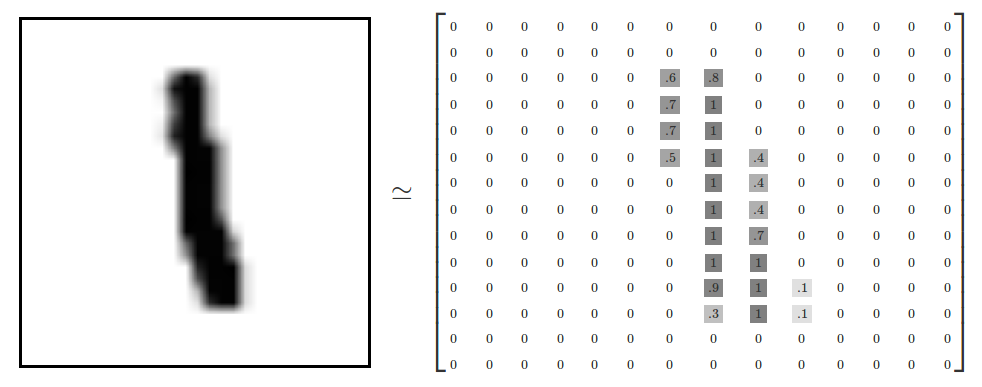
\includegraphics[scale=0.43]{Bilder/MNIST-Matrix}
	\caption{Eingabe in das neuronale Netzwerk.} 
	\label{fig:MNIST-Matrix} 
\end{figure}

\begin{figure}[!hbt]
	\centering
	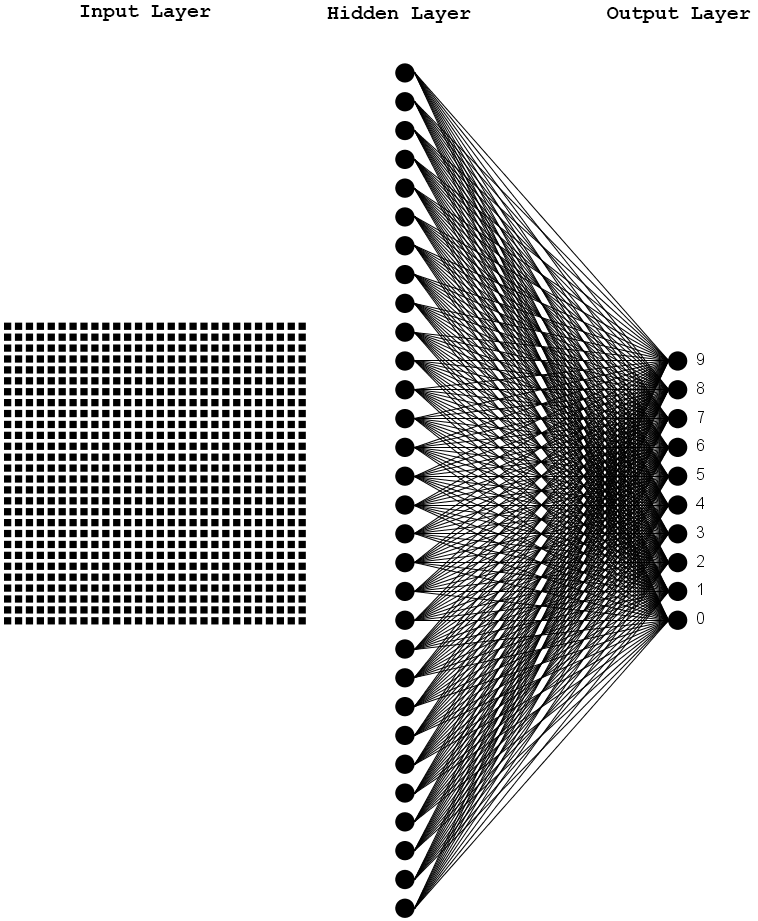
\includegraphics[scale=0.75]{Bilder/animation_network_default}
	\caption{Default Animation, welche über die Eingabe mit dem Wert $0$ aufgerufen wird.} 
	\label{fig:animation_network_default} 
\end{figure}
 
\noindent
Für die weitere Betrachtung der anderen Eingabebefehle soll zunächst das verwendete Farbmodell erläutert werden. Hierbei findet das additive Farbmodell im RGB-Farbraum seine Anwendung, wobei die Farbtiefe durch den jeweiligen Wert aus den Testdaten oder den Gewichtungen vorgegeben wird. Kleine Werte weisen im Vergleich zu größeren Werten einen höheren Weiß-Anteil auf. Die Einfärbungen im Untersuchungsbereich sind wie folgt definiert:
\begin{center}
\begin{tabular}{lp{6cm}}
\textbf{Farbe}   & \textbf{Erklärung} \\
\hline \\
blau, grün & Bereich mit einer geringen Relevanz \\[0.2cm]
rot, gelb  & Bereich mit einer hohen Relevanz   \\
\end{tabular}
\end{center} 
\vspace{1cm}

\noindent
Die \textbf{Eingabebefehle 1 - 30} betrachten den Untersuchungsbereich eines einzelnen Neurons der verborgenen Schicht, welches hierbei bei der Auswahl farblich hervorgehoben wird. Der Untersuchungsbereich ist farblich in rote und blaue Bereiche aufgeteilt. Pixel mit einer roten Färbung, haben eine hohe Gewichtung. Dahingegen weisen Pixel mit einer blauen Färbung einen geringen Gewichtungsfaktor auf. Blassere Farben haben hierbei eine geringere Merkmalsausprägung. Die Animation weist hierbei den folgenden Aufbau auf (siehe Abb. \ref{fig:untersuchungsbereich_neuron}). \\

\begin{figure}[!hbt]
	\centering
	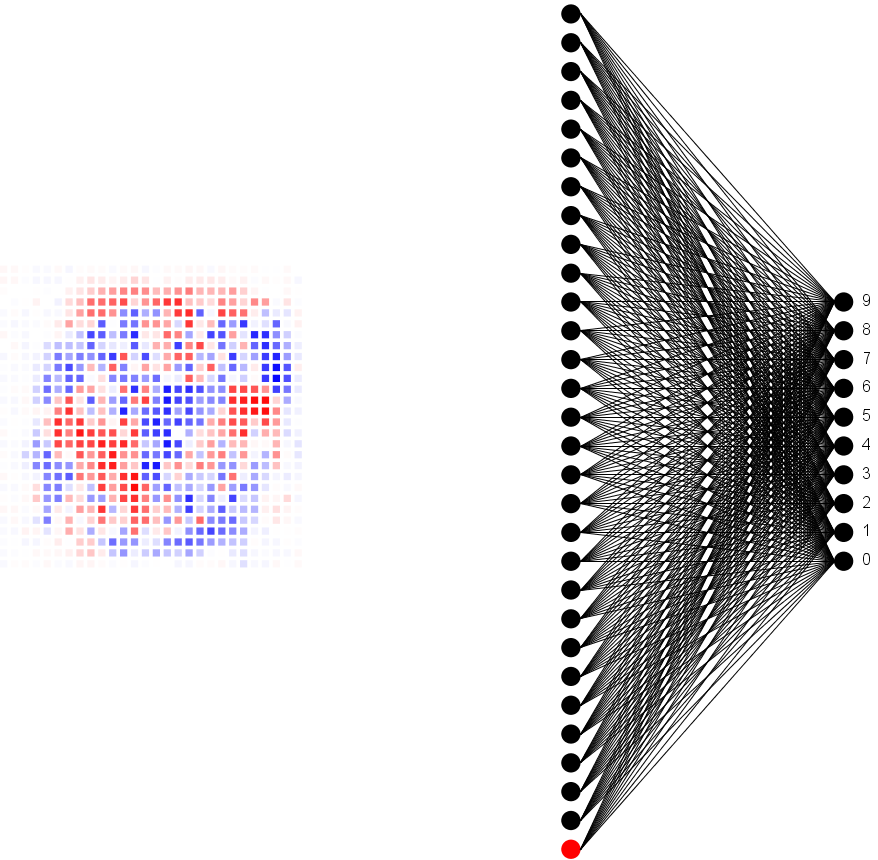
\includegraphics[scale=0.8]{Bilder/untersuchungsbereich_neuron}
	\caption{Untersuchungsbereich eines einzelnen Neurons der verborgenen Schicht.} 
	\label{fig:untersuchungsbereich_neuron} 
\end{figure}

\noindent
Über den \textbf{Eingabebefehl 1000} wird der Untersuchungsbereich von allen Neuronen in einer Übersicht abgebildet. Dies bedeutet, dass dieser Befehl die Ausgaben von den Eingabebefehlen 1-30 in sich zusammenfasst (siehe Abb. \ref{fig:untersuchungsbereich_neuronen}). Die grafische Ausgabe ermöglicht dem Anwender die Untersuchungsbereiche verschiedener Neuronen zu vergleichen und gegenüberzustellen. Konzentriert sich ein Neuron im Vergleich zu allen anderen nur auf einen bestimmten Bereich? Nimmt ein Neuron für die Erkennung einer handgeschrieben Zahl (z.B. $6$) einen größeren Einfluss wie andere Neuronen? \\

\begin{figure}[hbt]
	\centering
	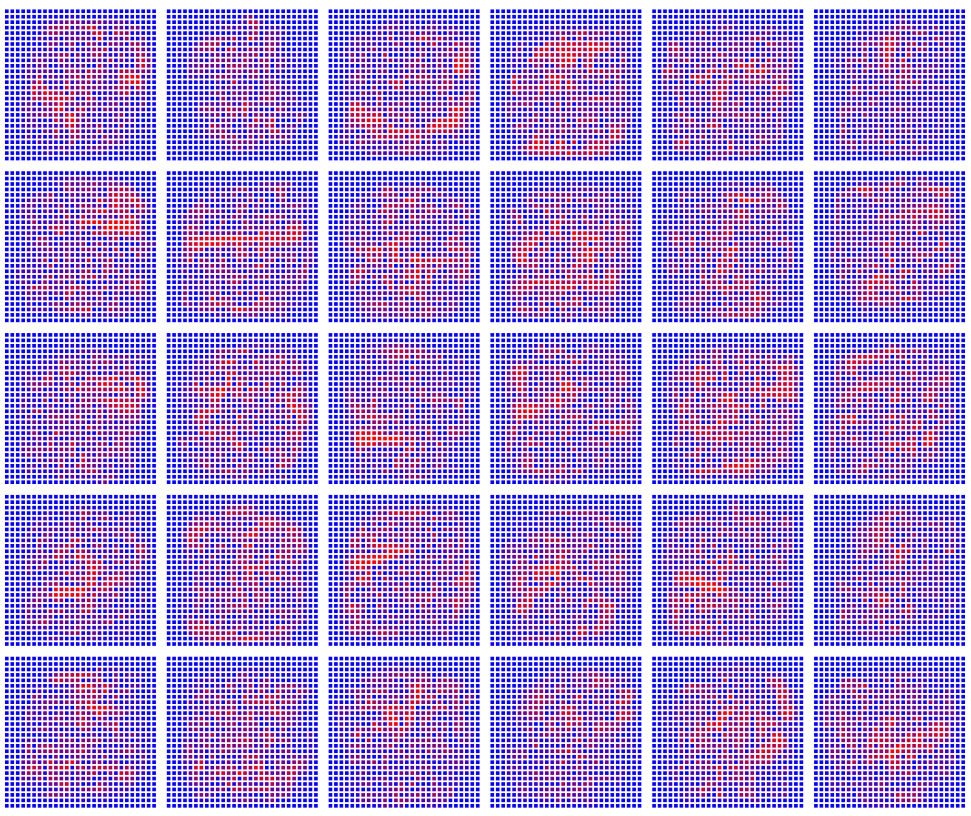
\includegraphics[scale=0.7]{Bilder/untersuchungsbereich_neuronen}
	\caption{Untersuchungsbereich aller Neuronen der verborgenen Schicht.} 
	\label{fig:untersuchungsbereich_neuronen} 
\end{figure}

\noindent
Der letzte \textbf{Eingabebereich 101-Datensatzgröße} ermöglicht den Untersuchungsbereich der Neuronen hinsichtlich einer Eingabe aus den Trainingsdaten zu betrachten. Des Weiteren wird das Untersuchungsobjekt, die Eingabe, sowie die Ausgabe mit dem berechneten Ergebnissen in der Animation abgebildet (siehe Abb. \ref{fig:untersuchungsbereich_zahl}). Die berechneten Ergebnisse ermöglichen dem Nutzer zu überprüfen, ob die Klassifizierung durch das neuronale Netzwerk richtig vorgenommen wurde und welche Neuronen in bei der Ergebnisfindung höheren Einfluss nehmen. Die Berechnung unter jedem Untersuchungsbereich ist durch die Sigmoid-Funktion bestimmt. \\

\noindent
An dieser Stelle soll angemerkt sein, dass aufgrund der Verwendung von nur einer verborgenen Schicht in diesem Versuchsaufbau und der Anzahl von nur 30 Iterationen keine Erkenntnisse anhand der grafischen Ausgaben getroffen werden können. Hierzu müsste ein \textit{Multilayer-Network} mit einer wesentlichen höheren Anzahl von Iterationen implementiert werden.

\begin{figure}[hbt]
	\centering
	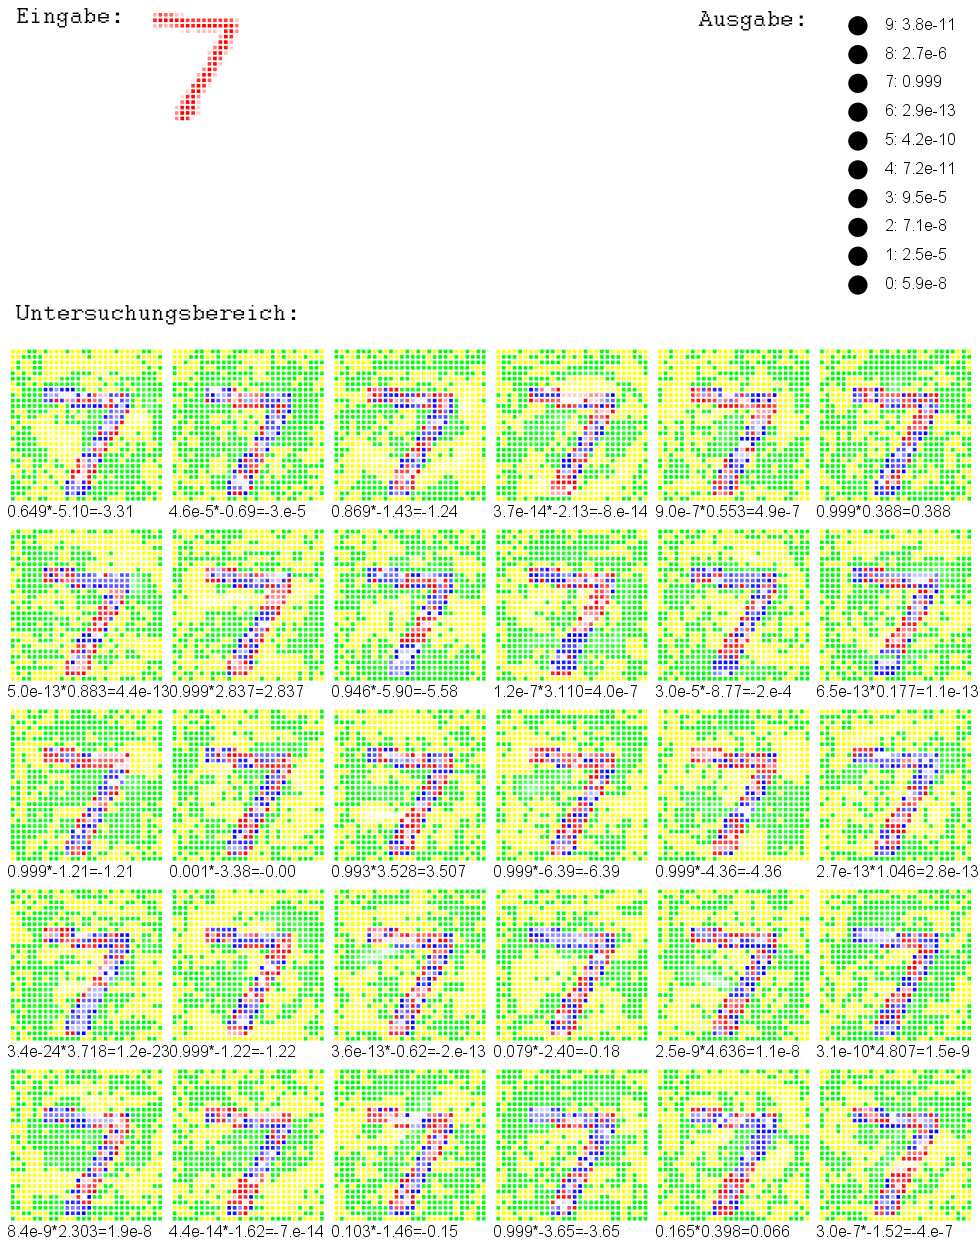
\includegraphics[scale=0.56]{Bilder/untersuchungsbereich_zahl}
	\caption{Untersuchungsbereich aller Neuronen der verborgenen Schicht hinsichtlich einer Eingabe.} 
	\label{fig:untersuchungsbereich_zahl} 
\end{figure}
